\documentclass{nature}
\usepackage{graphicx}	
\usepackage{amssymb}
\usepackage{amsmath}
\usepackage{algorithm2e}
\RestyleAlgo{ruled}
\usepackage{bbm}
\usepackage{geometry}
\usepackage{afterpage}
\usepackage{nonfloat}
\usepackage{lipsum}
\usepackage{nameref}
\usepackage[colorlinks=true,citecolor=blue,linkcolor=blue]{hyperref}
\newcommand\independent{\perp \!\!\! \perp}
\usepackage{capt-of}

\bibliographystyle{naturemag}

\title{Robust differential expression testing for single-cell CRISPR screens}

\author{Timothy Barry$^{1}$, Kathryn Roeder$^{1,2}$, and Eugene Katsevich$^{3}$}

\begin{document}
\maketitle
\addtocounter{page}{-1}
\thispagestyle{empty}

\clearpage


% Figure 1
  \includegraphics[width=\linewidth]{figures/fig_1_gene_v2.png}

\clearpage

% Figure 1
\afterpage{
  \centering
  \includegraphics[width=\linewidth]{figures/fig_1_gene_v3.png}
  \figcaption[Short caption text for the list of figures]{Insert caption here.}
  \label{fig:undercover}
  \hrulefill
}

% Figure 2
\afterpage{
  \centering
  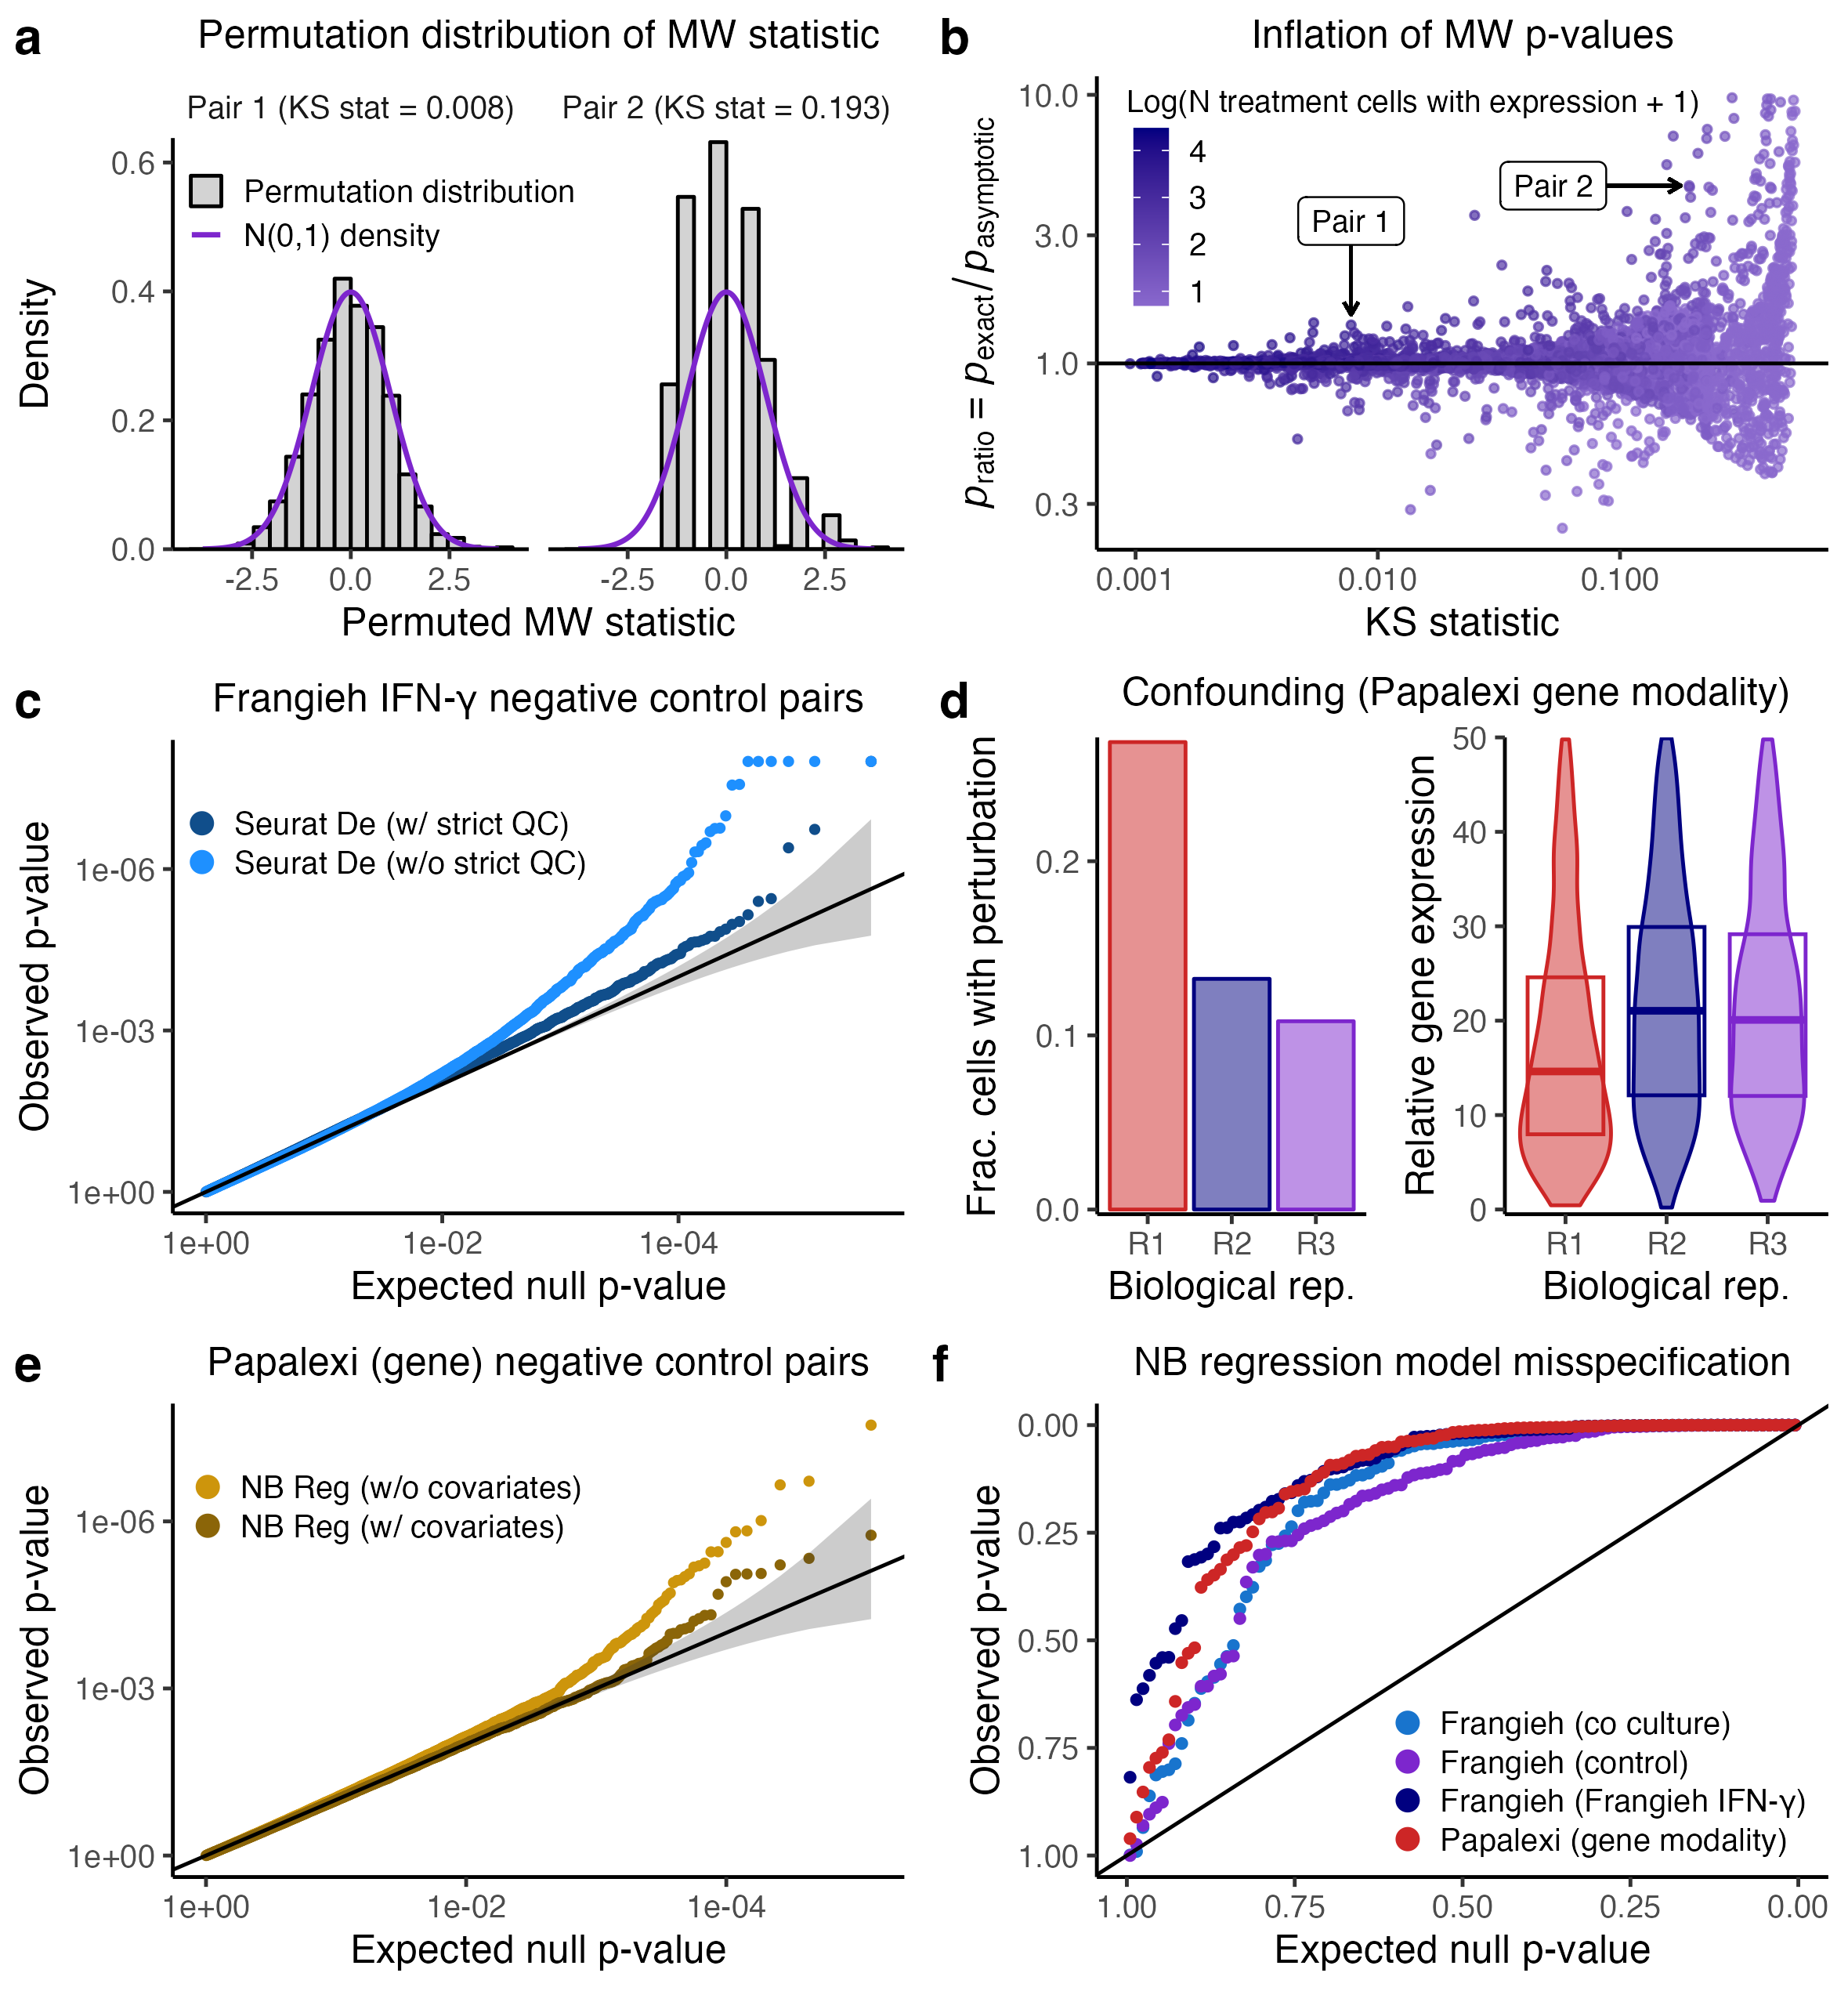
\includegraphics[width=1.0\linewidth]{figures/fig_2.png}
  \figcaption[Short caption text for the list of figures]{\textbf{Sparsity, confounding, and model misspecification are core analysis challenges in single-cell CRISPR screen analysis}. \textbf{a}, The exact null distribution of the Mann–Whitney (MW) test statistic (obtained via permutations; grey) on two pairs from the Frangieh IFN-$\gamma$ data. The MW test (and thus Seurat DE) approximates the exact null distribution using a standard Gaussian density (purple). For pair 1 (left), the Gaussian approximation to the exact null distribution is good (KS statistic = 0.008); for pair 2, by contrast (right), the approximation is poor (KS statistic = 0.193). \textbf{b}, A plot of $p_\textrm{ratio}$ (defined as the ratio of the exact MW p-value, $p_\textrm{exact}$, to the asymptotic MW p-value, $p_\textrm{asymptotic}$) vs.\ goodness of fit of the Gaussian distribution to the exact null distribution (as quantified by the KS statistic). Each point represents a gene-gRNA pair; pairs 1 and 2 (from panel \textbf{a}) are annotated. As the KS statistic increases (indicating worse fit of the Gaussian distribution to the exact MW null distribution), $p_\textrm{ratio}$ deviates more from one, indicating miscalibration. Points are colored according to the effective sample size (as quantified by the number of treatment cells with nonzero expression) of the corresponding pair. \textbf{c}, An application Seurat DE to the IFN-$\gamma$ negative control data with and without stringent QC; applying stringent QC in this context amounts to filtering for pairs with with a very large effective sample size. \textbf{d}, An example of confounding on the Papalexi data. Left (resp. right), the fraction of cells that received a given NT gRNA (resp., the relative expression of a given gene) across biological replicates ``R1,'' ``R2,'' and ``R3.'' If we failed to account for biological replicate, we would conclude (incorrectly) the the NT gRNA \textit{decreases} the relative expression of the gene. \textbf{e}, Application of NB regression to the Papalexi data. Inclusion of confounders (such as biological replicate) in the regression model improves calibration (although further improvements are possible). \textbf{f}, A QQ-plot of p-values obtained from testing for goodness of fit of the NB regression model to the gene expression data (points colored by dataset). The p-values are inflated, indicating that the NB regression model provides a poor fit to some subset of the genes.}
  \label{fig:analysis_challenges}
  \hrulefill
}

% Figure 4
\afterpage{
  \centering
  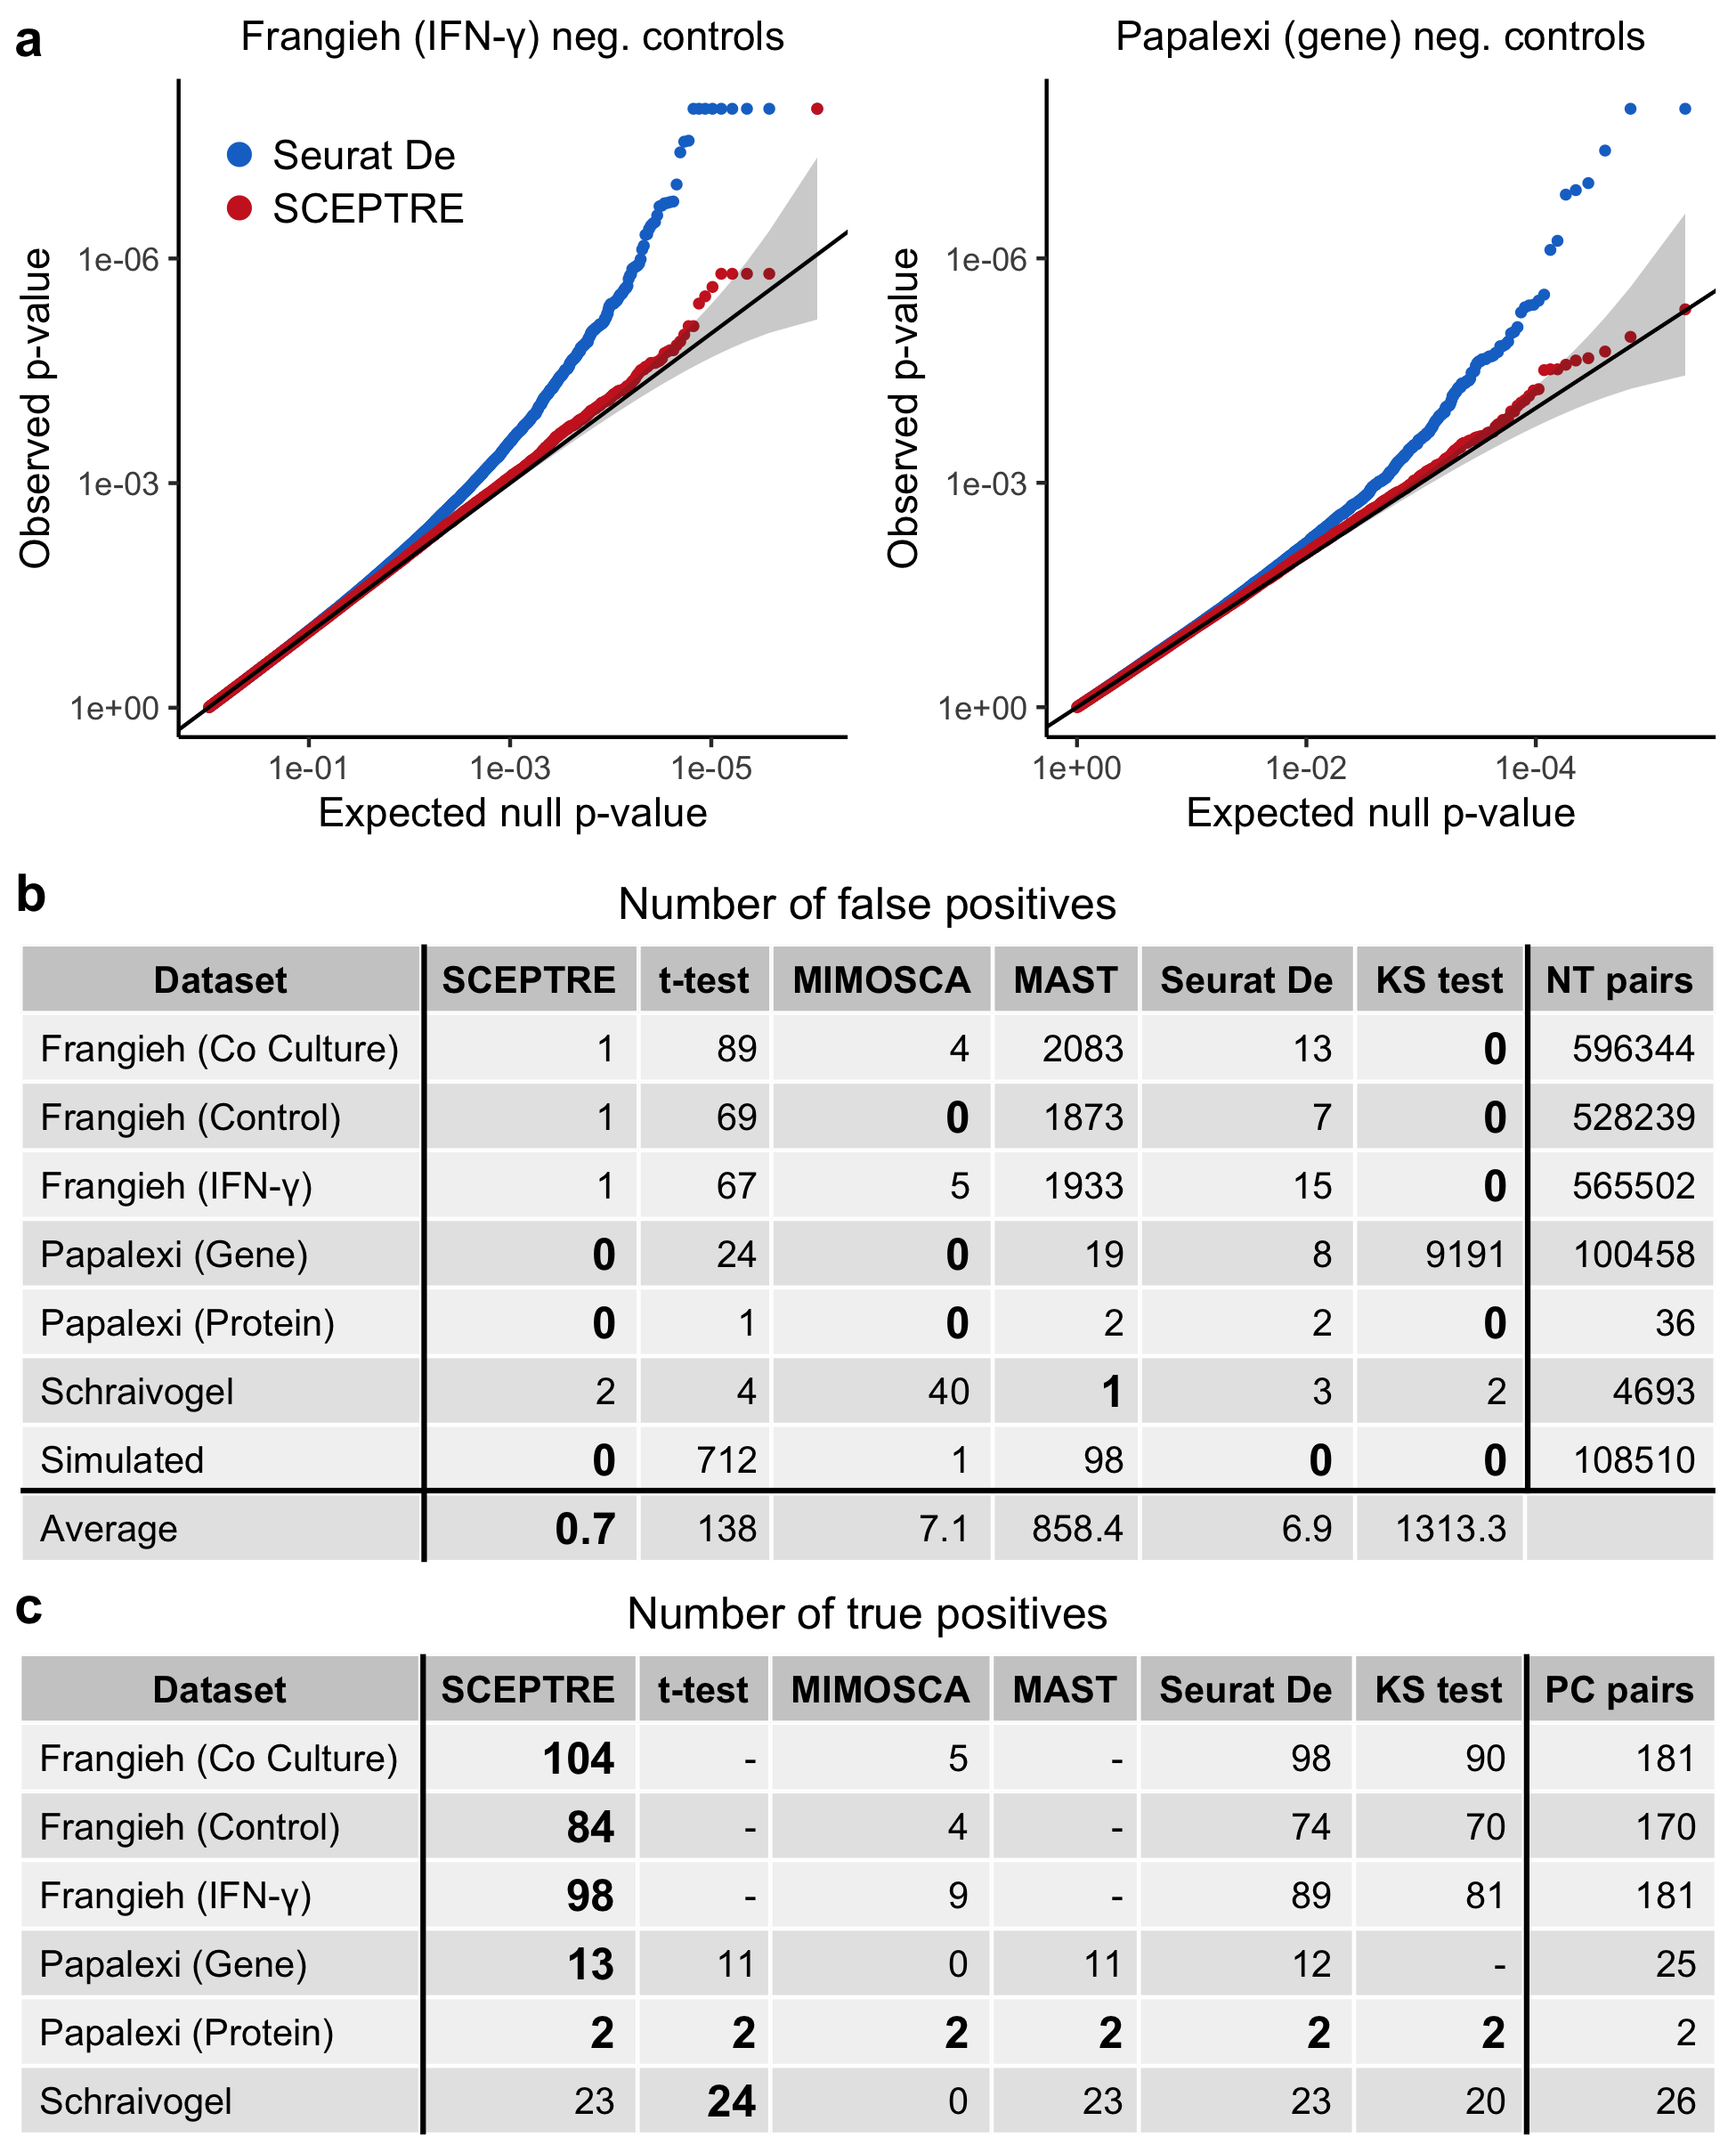
\includegraphics[width=\linewidth]{figures/fig_4_gene.png}
  \figcaption[Short caption text for the list of figures]{Insert caption here.}
  \label{fig:sceptre_results}
}

\end{document}
